\documentclass[a4paper,12pt]{report}
  \usepackage[english]{babel}
  \usepackage{graphicx}
  \linespread{1.5}
  \title{Implementation and Evaluation of Routing Algorithm in GENI Software-Defined Networking}
  \author{Wei-Hen Hsu}
  \date{\today}
  \begin{document}
  \begin{large}
  \maketitle{}
  \tableofcontents{}
  \chapter{Introduction}
	    \qquad Software-defined networking (SDN) has received a lot of attention in recent years, 
	            several routing algorithms have been proposed by researchers. The environment that evaluates a 
	            routing algorithm is quite importmant.\par
	    \qquad Commonly, building up a SDN environment with real OpenFlow switches for evaluating the porformance
	            of routing algorithms is very persuasive. Unfortunately, a real OpenFlow switch is expensive. It's 
	            costly to build a small-scale netwrok with real OpenFlow switches.\par
	    \qquad Another tool for building the SDN environment is the network testbed. The network testbed is a 
	            platform to provide network researchers with a realistic environment for testing. In some network testbeds, they are supported by governmentsit and it's free for researchers to use the testbed. Compared with previous ways, it is more cost-effective for researchers to build the environment.\par
	    \qquad Therefore, in this thesis, we propsed a method to implement the routing algorithms in {\bf Global 
	            Environment for Network Innovations (GENI)} SDN testbed. The routing algorithms fall into the following two main categories: (a) online routing algorithm; (b) offline routing algorithm. In each catergory, we describe the process of creating a SDN on GENI and implementing the rouing algorithm on SDN. 
  \chapter{General Background Information}
    \section{Software-defined networking}
      \qquad According to {\bf ONF(Open Networking Foundation)} definition of software-defined networking, SDN is 
                an architecture that is dynamic, manageable, cost-effective, and adaptable, making it ideal for the 
                high-bandwidth, dynamic nature of today’s applications. In traditional network, each network device 
                usually has its own control plane. The transport of the packet is processed by network device 
                individually. The SDN decouples the forwarding and control planes, removes the control plane from 
                network device and implements it in sofware instead. The SDN enables the control plane to beccome 
                directly programmable and the underlying infrastructure to be abstracted for applications and network 
                services. The OpenFlow® protocol is a foundational element for building SDN solutions.
    \section{OpenFlow}
      \qquad OpenFlow is a communication protocol between SDN controller and OpenFlow switch that enables the SDN 
                controller to direct interact with the forwarding plane of network devices such as switches and 
                routers. Figure 2.1 shows the main components of an OpenFlow switch.
        \begin{figure}[hb]
          \caption{Main components of an OpenFlow switch.}
          \centering
            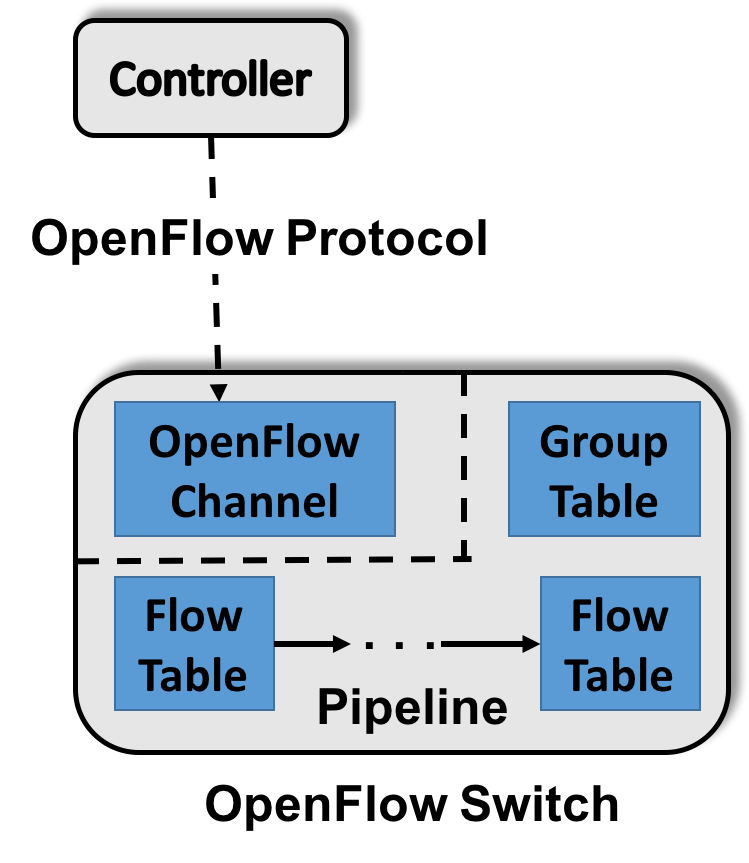
\includegraphics[width=0.5\textwidth]{OpenFlow.png}
        \end{figure}
        \subsection{OpenFlow switch components}
        \qquad An OpenFlow switch consists one or more flow tables, which perform packet lookups and forwarding. The controller could use the OpenFlow protocol to add, update, and delete flow entries in flow tables. In each flow table, it contains a set of flow entries; each flow entry consists of match fields, counters, and a set of instructions to apply to matching packets. (see Table 2.1)\\
        \begin{table}
          \centering
          \begin{tabular}[c]{|l|l|l|l|l|l|}
          \hline
          Match Fields & Priority & Counter & Instructions & Timeouts & Cookie \\
          \hline
          \end{tabular}
          \caption{Main components of a flow entry in a flow table}
        \end{table}
      \section{GENI}
      \qquad GENI provides a virtual laboratory for networking and 		 distributed systems research and education.Researcher could obtain compute resources from locations around the United States. Figure 2.2 show the map of GENI compute and netwrok resouces. GENI allows user to install custom software or even custom operating systems on compute resources. Furthermore, researcher could control how network switches in their experiment handle traffic flows. GENI is sponsored by the U.S. National Science Foundation (NSF). If the researchers' institution belongs to an identity federation, the researchers are able to log in using their usual username and password. If their institution does not belong, they could apply for an account at the NCSA identity Provider.
      \begin{figure}[h]
          \caption{The map of GENI compute and netwrok resouces.}
          \centering
            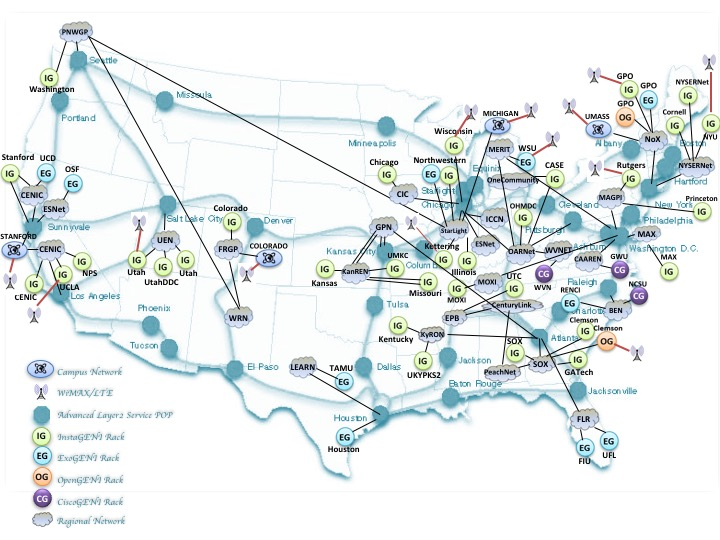
\includegraphics[width=1.0\textwidth]{GENI-MAP.jpg}
      \end{figure}
     \section{Open vSwitch}
     \qquad Open vSwitch is a open source, multi layer virtual switch implemented in software. It can be intergrated with hardware where it can act as as control plane. One example is it can handle OnpenFlow control plane in a hardware silicon. There are three mainly components in Open vSwitch: (a) Control Plane; (b) Kernel Mode; (c) Command line interface. 
     \section{Ryu controller}
     \qquad Ryu is a component-based SDN framework. Ryu is fully written in Python and provides software components with well defined API that make it easy for developers to create new management and control applications. 
     \chapter{System model}
     \section{Workflow of GENI}
     \qquad Figure 3.1 shows the workflow of GENI. In the beginning, the GENI experimenters need to creat a slice. A GENI slice is: (a) The unit of isolation for experiments. Only experimenters who are members of a slice can make changes to experiments in that slice; (b) A container for resources used in an experiment.
     \newline
     \null\qquad For creating a specific topology, there are three methods to achieve that. Resouece Specification (RSpec) is a XML document in a prescribed format. Experimenters sned to  aggregates a request RSpec that describe the rosources they want.\
     \newline
     \null\qquad After finishing in reservation, experimenters could use GENI desktop tool to configure each node manually. Another method is to use the manifest RSpec, manifest RSpec describes the roesources the got. The manifest include the names and IP addresses and login accounts of compute resources. The experimenters could use SSH to login in the resources and configure the nodes.
     \newline
     \null\qquad When finished setting the nodes including controller, the experimenters use SSH to connect to each node and run the {\bf iPerf} to start the traffic. {\bf iPerf} is a software that could create the traffic in the networks \cite{iperf}.
     \newline
     \null\qquad Finally, the experiments could clone the mesaurment datas from each node and view the information they want.
       \begin{figure}
          \caption{The workflow of GENI.}
          \centering
          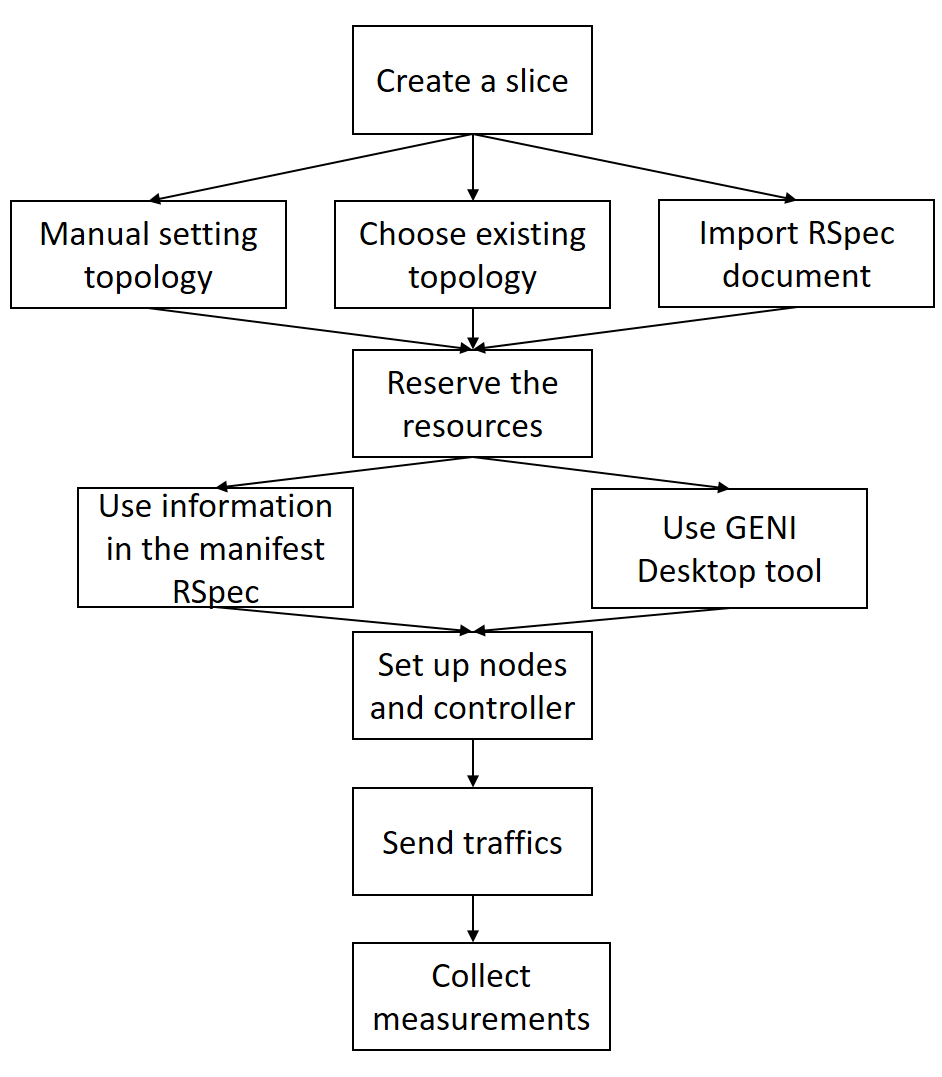
\includegraphics[width=1.0\textwidth]{geni_workflow.png}
       \end{figure}
	    \section{Network in GENI}
	      \qquad Figure 3.2 shows the network in GENI. Each nodes is a virtual machine installed the Open vSwitch. The controller is installed the RYU controller.
	    \begin{figure}
	          \caption{The network in GENI.}
	          \centering
	          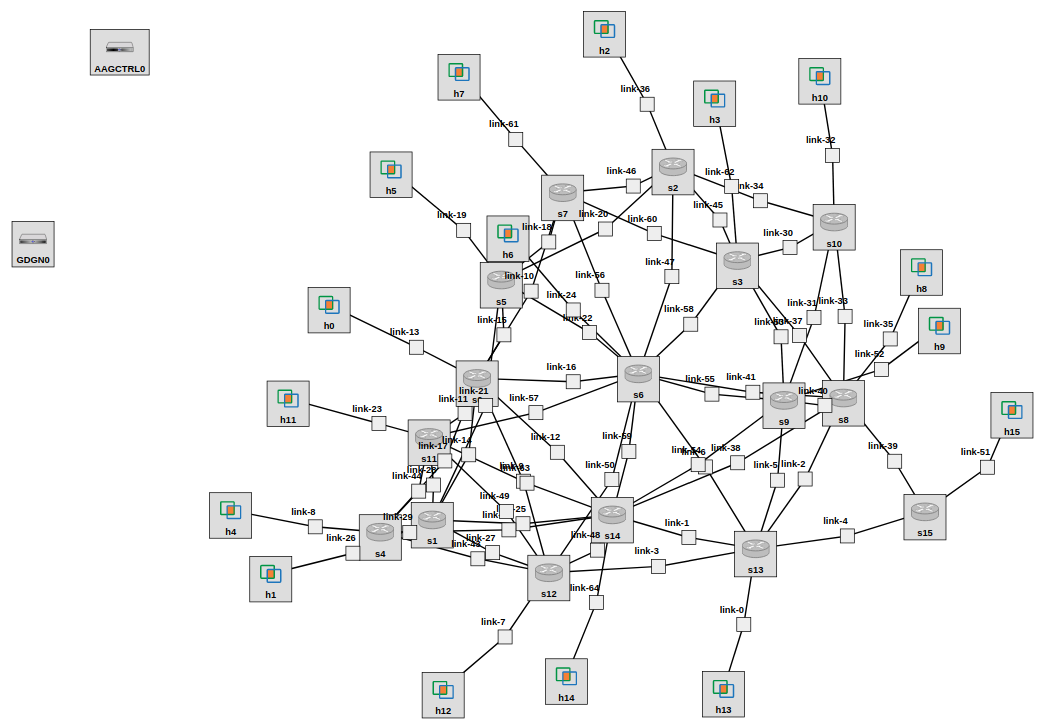
\includegraphics[width=1.0\textwidth]{GENI_network.png}
	       \end{figure}
	    \section{Ryu controller}
	    \qquad In Ryu controller, the controller will make connection to each switch by using OpenFlow protocol to send the hello message. After receving the reply message, the controller will want to get the information of switches. The controller will send the features request to the switch and wait the reply message. Then, the controller will send to flow mod message to the switch which setting the switch how to handle the packet. After that, the controller will start to listen the packet. When a packet is sent to the controller by the switch. The controller will create an event. Because the event is casue by a pcket being sent, so the evnet will be sent to the function which handle with the packet in controller.Figures 3.3 shows the model of Ryu application. The data path thread will collect all the events from OpenFlow switch and dispatch the events to the event handler to process it. The programmer should define the event handler how to process the event. Figure 3.4 shows the status of ryu from the beginning till the end. Figure 3.5 is a example code of how the controller handling the packet.
	     \begin{figure}[p]
	          \caption{Ryu application programming model.}
	          \centering
	            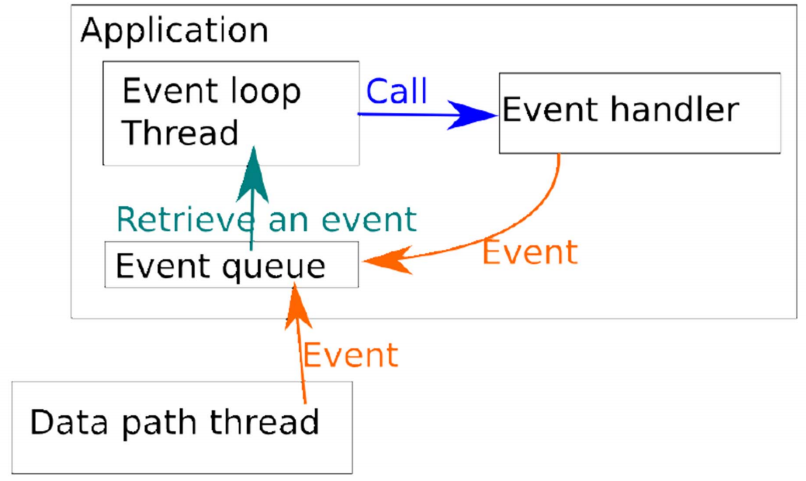
\includegraphics[width=1.0\textwidth]{ryu_model.png}
	          \caption{The four status in ryu controller}
	          	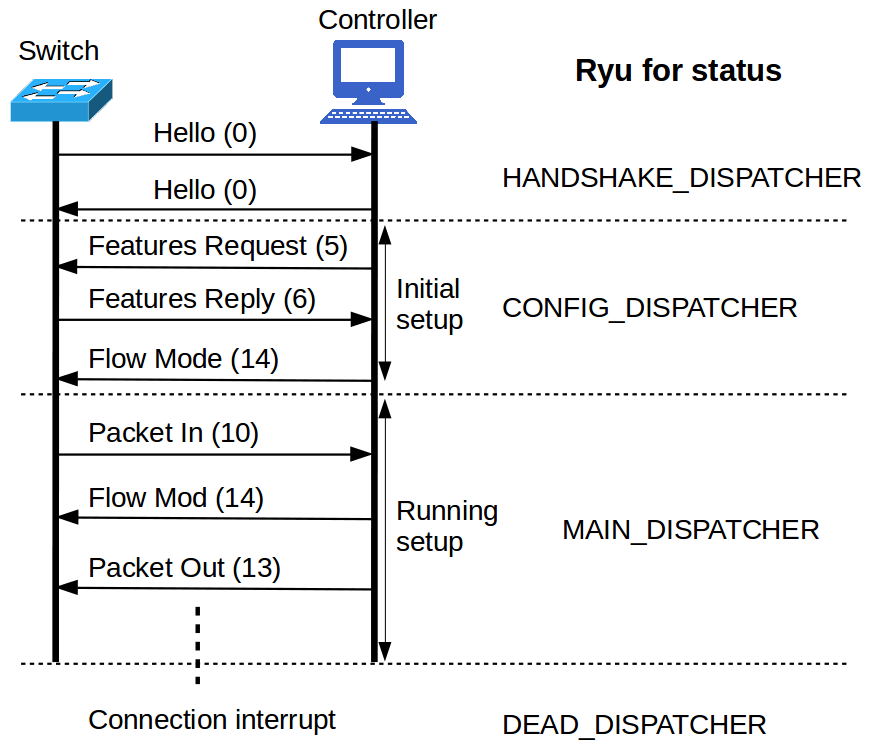
\includegraphics[width=1.0\textwidth]{ryu_graph.png}
	          
	      	\end{figure}
	     \begin{figure}[p]
	          \centering
	          \caption{The example of the function which handle the packet}
	          	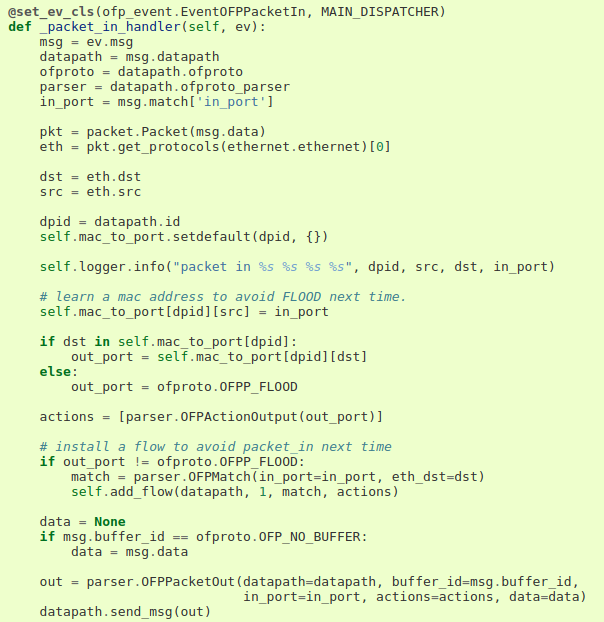
\includegraphics[width=1.0\textwidth]{packet_in_handler.png}
	      	\end{figure}
  \chapter{Implementation of Routing Algorithm in GENI}
	  	\section{The reservation of compute resources for customized topology}
			\qquad In GENI, There are three methods to reserve the resources: (a) setting the topology manually; (b) choose existing topology; (c) import Resouce spectification (Rspec) documents. Figure 4.1 to Figure 4.3 show the three methdos to reserve the resources. In (a), you could just drag the components into the screen and create the topology you desire. In (b) choosing the existing topology that the geni offering. In (c) To use the Rspec documents, you could write a program to output the Rspec document by following the Rspec structure.
			\begin{figure}
	          \caption{(a) Setting the topology manually.}
	          \centering
	            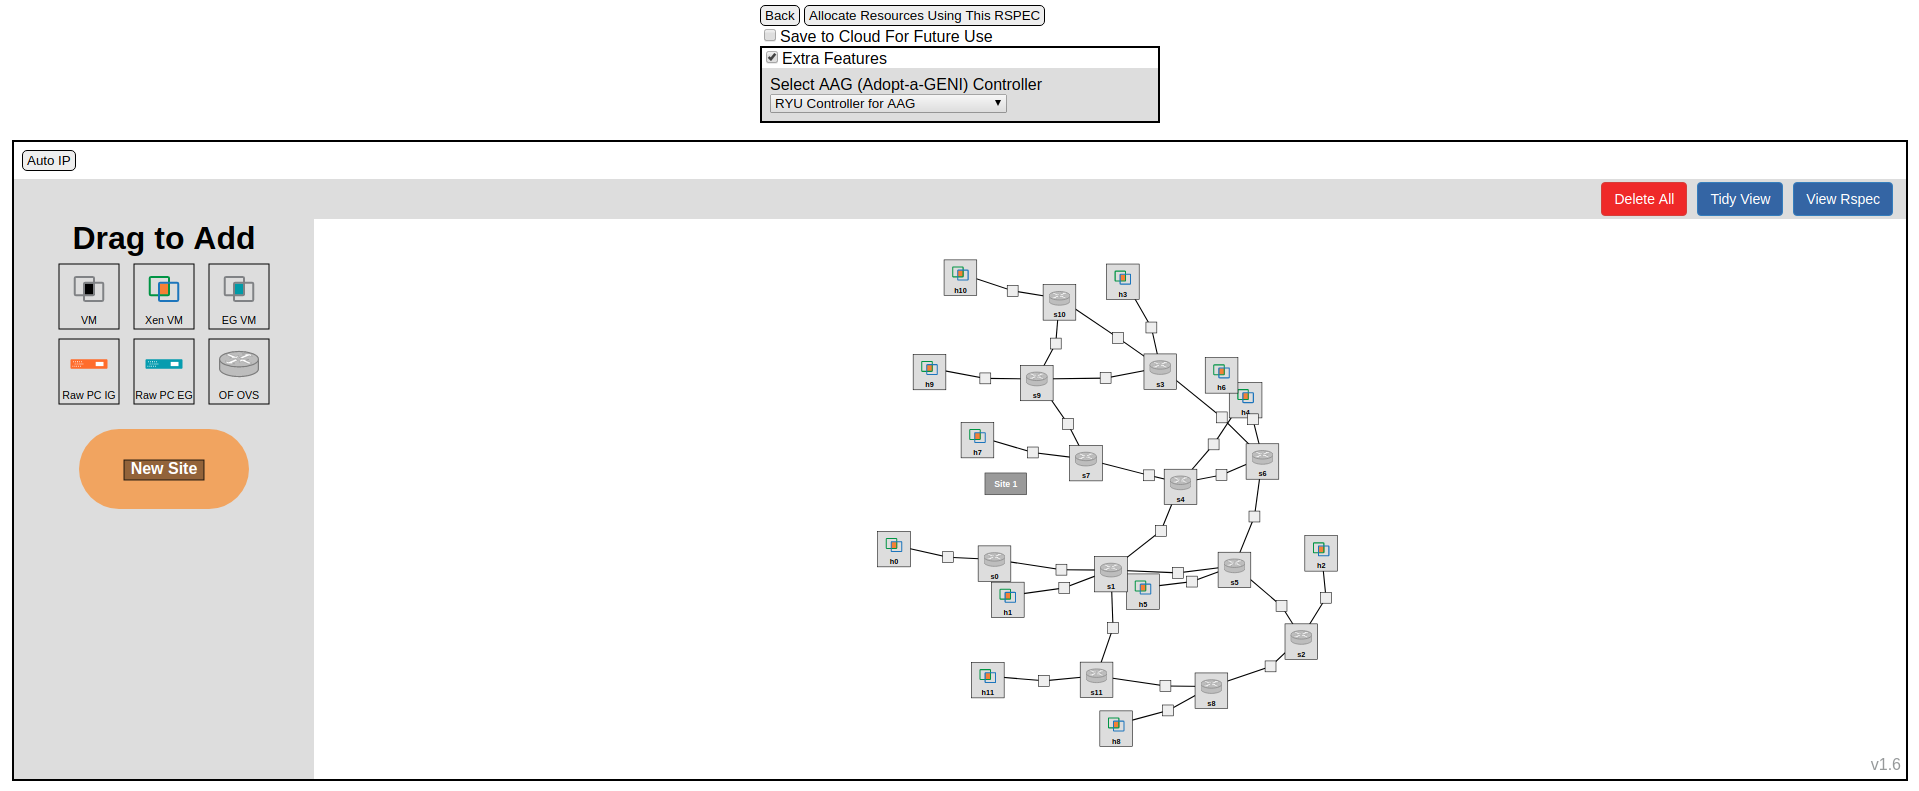
\includegraphics[width=1.0\textwidth]{geni_manual.png}
	          \caption{(b) Choose existing topology.}
	            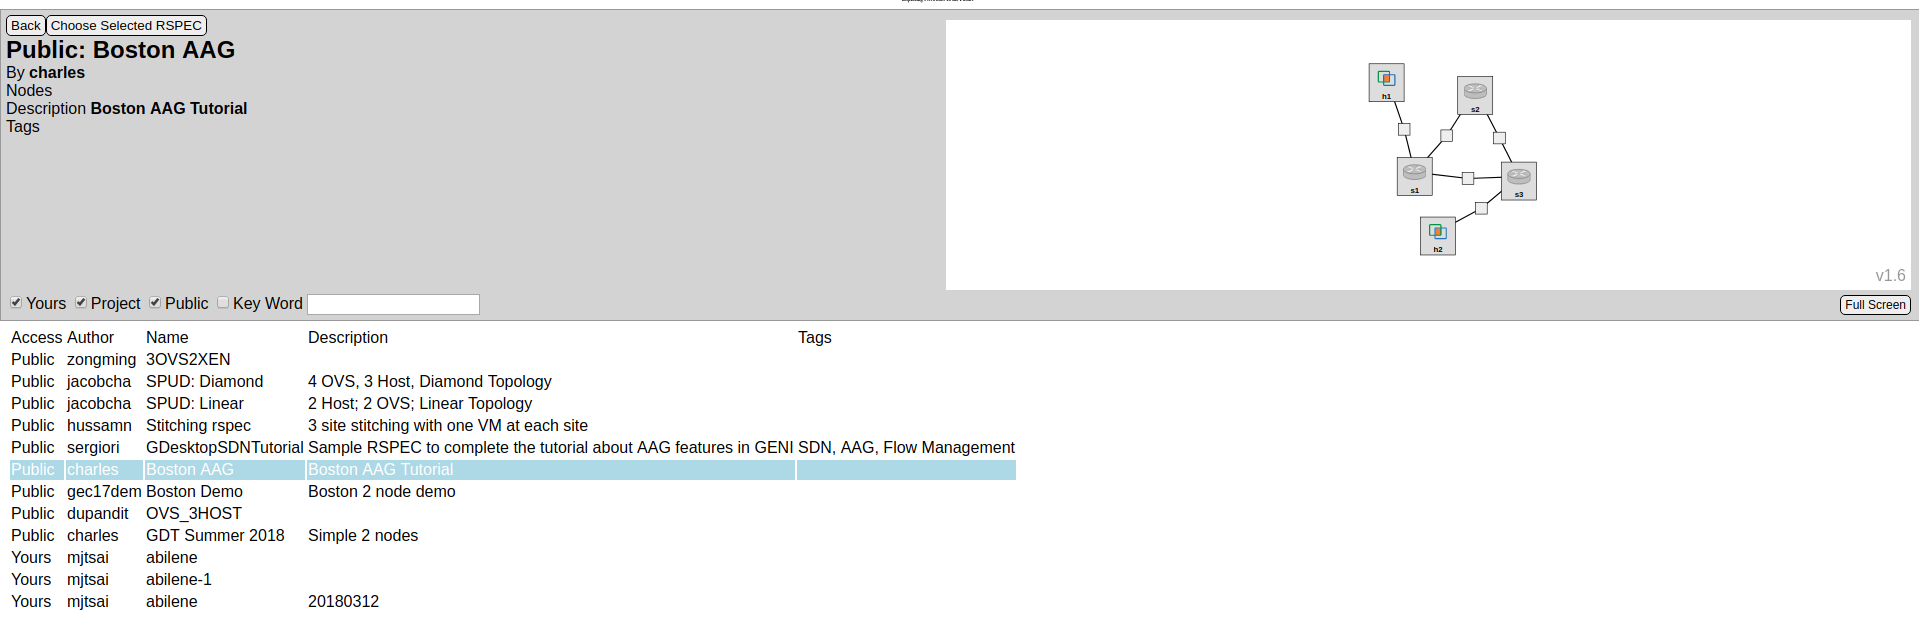
\includegraphics[width=1.0\textwidth]{choose_existing.png}
	          \caption{(c) Import Resouce spectification (Rspec) documents.}
	            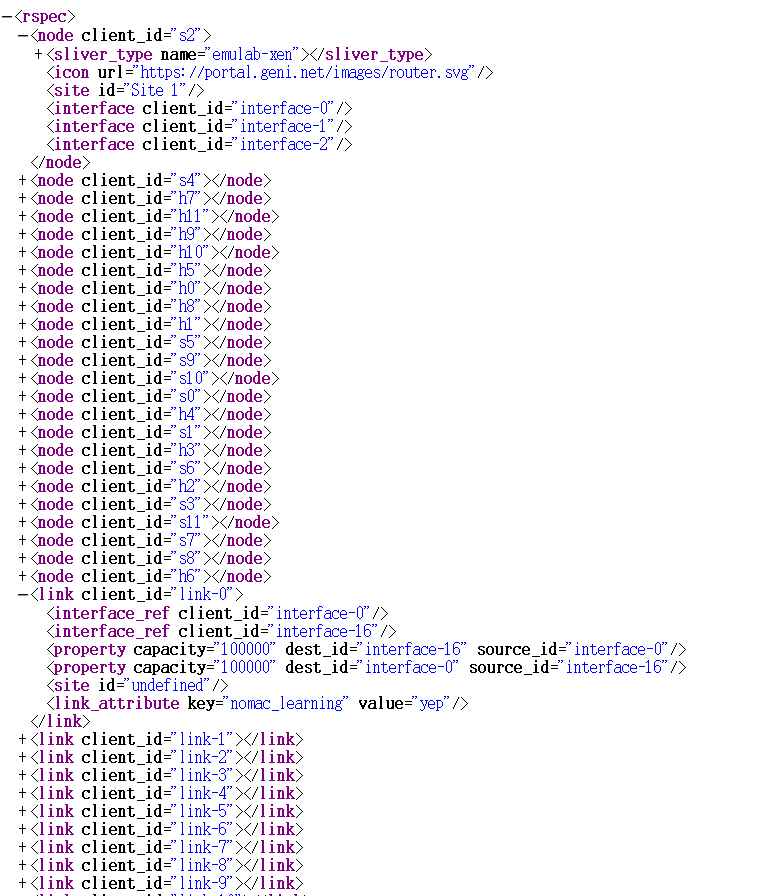
\includegraphics[width=1.0\textwidth]{rspec_format.png}
	      	\end{figure}
	   \section{Offline algorithm}
	     \subsection{create the network graph for the input of routing algorithm}
	     \qquad After reserving the resources, copy the network structure document from GENI online website. Fugure 4.4 shows the the network structure document. The network structure document contains the information of nodes and links. Using this document to create the netowrk graph for the input of the routing algorithm.
	     \begin{figure}
	        \caption{The network structure in GENI}
	        \centering
	          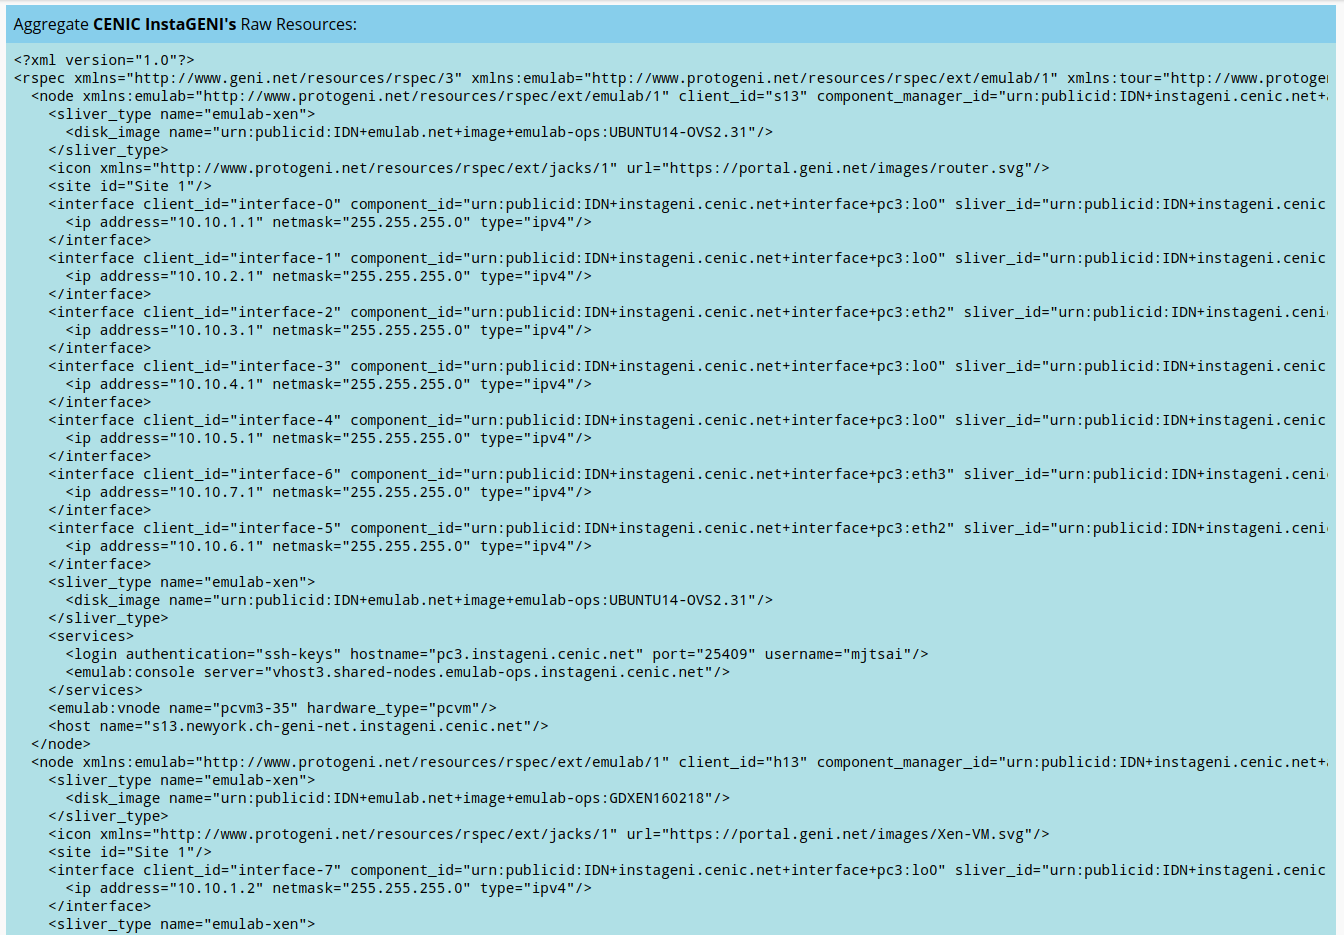
\includegraphics[width=1.0\textwidth]{Raw_resource.png}
	     \end{figure}
	     \subsection{setting up the demands}
	     \qquad After the routing algorithm compute the pathes of the demands. In order to let the Open vSwitch to identify each demands, we use ip of source, ip of destination, port of destination to identify each demands.
	 For each nodes, we create a script to run the demands with given information. 
	 	\subsection{setting up the controller}
	 	\qquad For controller, we create a dictionary for it. Every time when a node asks the controller how to process the demands, controller could use ip of source, ip of destination, port of destination as a key to find the path of the demand then send the OpenFlow message to the switch for adding the flow into the flow table. 
	 	\section{Online algorithm}
	 		\subsection{ryu controller}
	 		\qquad In ryu controller, we need to implement a topology discovery which the routing algorithm could use. Figure 4.5 is the package which the Ryu controller need to import. Figure 4.6 is the code to discover topology. After the controller gets the topology, every time when a packet sends to the controller, we parse the information of the packet. Getting its ip source, ip destination, destination port as the demand's key. Input this key and topology into the algorithm then get the path output by controller. Sending the messages to the switch to add the flow in the flow table.
	 		\begin{figure}
	          \caption{Ryu controller import package for topology discovery.}
	          \centering
	            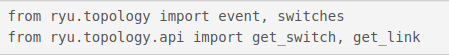
\includegraphics[width=1.0\textwidth]{ryu_import.png}
	          \caption{The code of topology discovery in Ryu controller.}
	            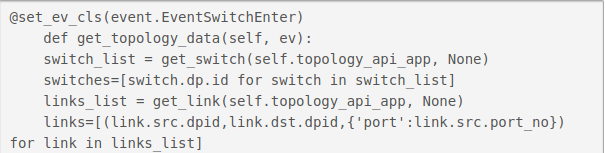
\includegraphics[width=1.0\textwidth]{ryu_discovery.png}
	      	\end{figure}
  \chapter{Case study}
  \section{Maximum Concurrent Flow Problem in MPLS-based Software Defined Networks}
    \qquad In this section, we study the Maximum Concurrent Flow Problem in MPLS-based Software Defined Networks and implement four algorithms in GENI. Because the MPLS is a per-flow routing, the number of flow paths through a node (switch) needs to be bounded due to the limited ternary content addressable memory (TCAM). Therefore, the problem term to be bounded forwarding rule maximum concurrent flow problem (BFRMCF)
    \subsection{Problem definition}
    \qquad Given a network topology $G=(V, E)$ with link link capacity (bandwidth capacity) $c_e\in R^+$ associated with each directed link $e\in E$ and node capacity (forwarding table size) $b_v\in Z^+$ associated with each node (SDN-FE) $v\in V$, and given a set of flows $F=\{ 1, 2, ..., |F|\}$. Each flow $f\in F$ is associated with a source-destination pair $ \left( s_f,t_f \right)\subseteq V \times V $ and the transmission demand $d_f \in R^+$. The Bounded Forwarding Rules Maximum Concurrent Flow Problem (BFRMCF) asks for the forwarding paths and the transmission rate on each chosen path such that 1) for each flow $f$, the rate is at least $\lambda d_f$, \newline 2) for each flow $f$, the rate is at most $d_f$ (the demand constraints), \newline 3) for each link $e$, the taotal rate through $e$ are at most $c_e$ (the link capacity constraints), \newline 4) for each node $v$, the number of flow paths going through $v$ does not exceed $b_v$ (the node capacity constraints), and \newline 5) $\lambda$ is maxized. \newline\null
\qquad Let $P_f$ be the set of possible forwarding paths for flow $f$ in the network, and $P=P_1 \cup P_2 \cup ... \cup P_F$. Moreover, let $c_p$ be the capacity of a path $p \in P_f$, i.e., $c_p = min\{ min_{e:e\in p} \{ c_e \}, d_f\}$. In addition, variable $x\left( p \right)$ deontes the fraction of the transmission rate on path $p$ to $c_p$, and variable $y\left( p \right) = 1$ if and only if $p$ is a chosen forwarding path. The BFRMCF problem is formulated as an integer linear program as below.
			\begin{figure}
	          \centering
	            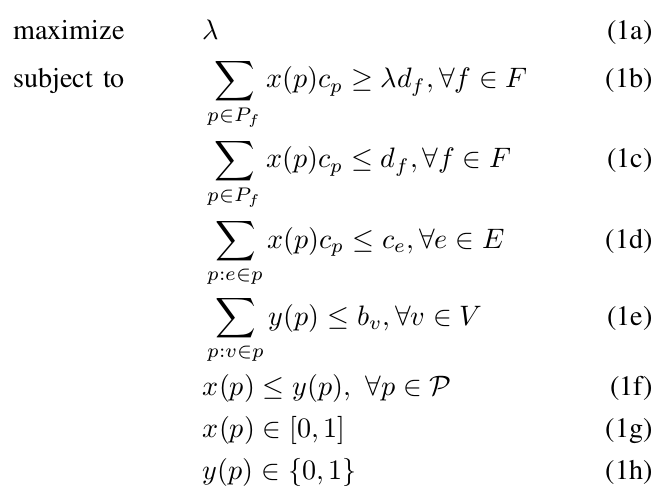
\includegraphics[width=1.0\textwidth]{it_program.png}
	      	\end{figure}
\section{Algorithms of BFRMCF}
\qquad We reivew three offline algorithms for BFRMCF problem. In \cite{our}, \cite{grag}, \cite{gk}, we implement it on GENI and show the total throughput and the $\lambda$ in rxperiment results.
\section{Implement method}
\subsection{ The ryu controller}
  \qquad In ryu controller we need to parse the packet to get the source of ip, destination of ip and destination of port for pretending as a key. Figure 5.1 is the code in ryu for parsing the packet.
  \begin{figure}[b]
	          \caption{The code of parse packet}
	          \centering
	            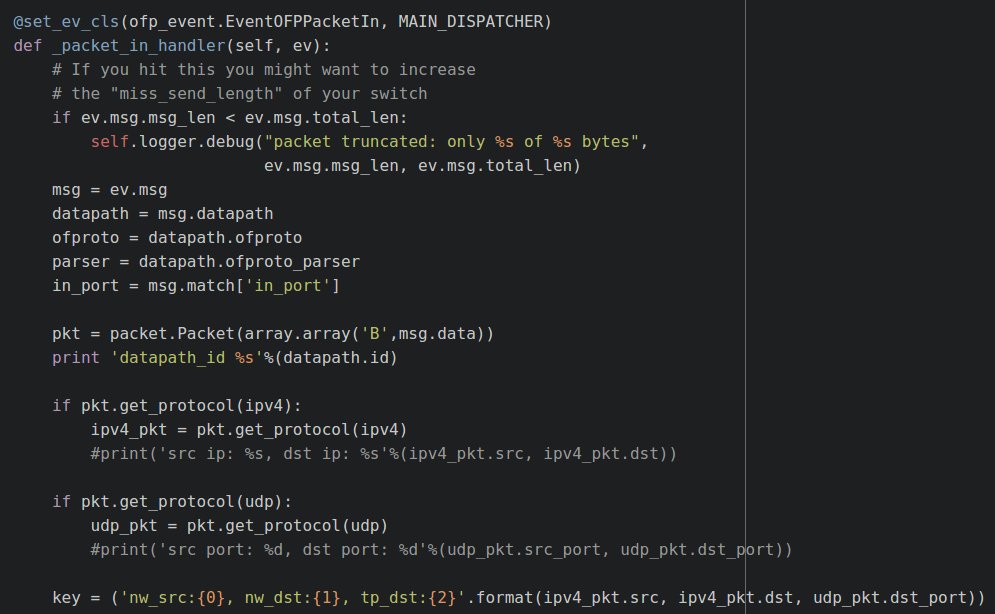
\includegraphics[width=1.0\textwidth]{ryu_controller_parse.png}
	      	\end{figure}
\subsection{ OpenFlw version and flow table size}	
\qquad In BFRMCF problem, because it has path degree constraint, we need to let the Open vSwitch support to 1.3 version and set up the flow limit. Figure 5.2, 5.3 is the code to set up. 
			\begin{figure}[b]
	          \caption{Support to OpenFlow 1.3}
	          \centering
	            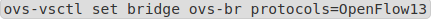
\includegraphics[width=1.0\textwidth]{openflow1_3.png}
	          \caption{Change flow table size}
	            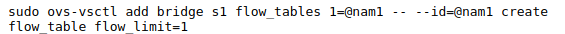
\includegraphics[width=1.0\textwidth]{flow_table.png}
	          \caption{The code of iPerf}
	          \centering
	            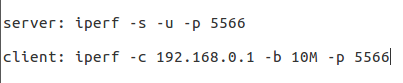
\includegraphics[width=1.0\textwidth]{iperf.png}
	      	\end{figure}
\subsection{iPerf}
	\qquad For setting a target bandwidth, because TCP couldn't fixed in a target bandwidth, so we selected UDP to transport. In figure 5.4, for server side, we user -p parameter to set up the server in a particular listen port, -u let the server listen for UDP packet.
	\newline\null\qquad For a client side, -c menas to be a client, -b is to set a target bandwidth. -p is transport to a particular listen port.
  \chapter{Experiment results}
  \qquad We tested three algorithms which are Garg’s algorithm \cite{grag}, Gushchin’s algorithm \cite{gk} and PD's algorithm \cite{our}.The network instances were obtained from the 6 real-life traces from SNDlib \cite{SNDlib}. Since the capacity of each node is unavailable, we set the switch capacity from the 0.1 number of demands($|K|$) to $1.0|K|$. The following figures show the  minimum fraction and total throughput in different topologys.
  \begin{figure}[ht]
    \caption{The impact of the switch capacity on the minimum fraction on GENI.}
	\centering
	  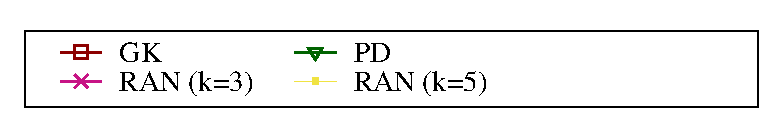
\includegraphics[width=1.0\textwidth]{lambda_legend.eps}
	  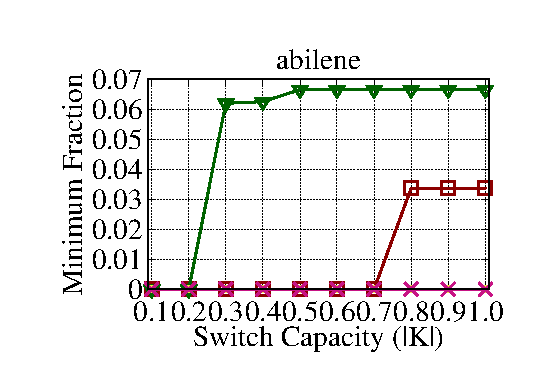
\includegraphics[width=1.0\textwidth]{abilene_geni_lambda_e05.eps}
	  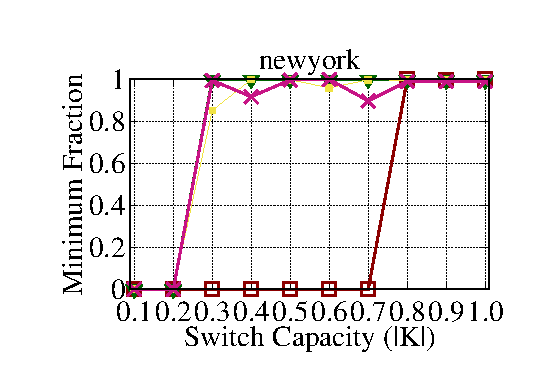
\includegraphics[width=1.0\textwidth]{newyork_geni_lambda_e05.eps}
  \end{figure}
    \begin{figure}[ht]
    \caption{The impact of the switch capacity on the minimum fraction on GENI.}
	\centering
	  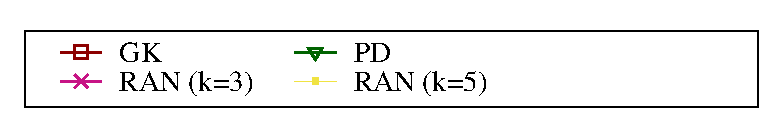
\includegraphics[width=1.0\textwidth]{lambda_legend.eps}
	  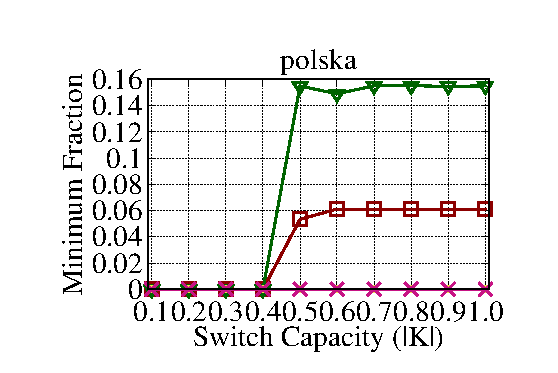
\includegraphics[width=1.0\textwidth]{polska_geni_lambda_e05.eps}
	  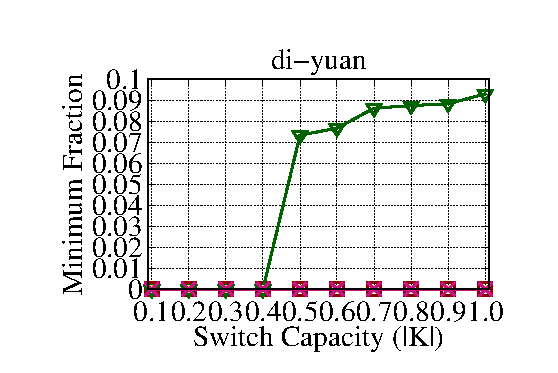
\includegraphics[width=1.0\textwidth]{di-yuan_geni_lambda_e05.eps}
  \end{figure}
  \begin{figure}[ht]
    \caption{The impact of the switch capacity on the minimum fraction on GENI.}
	\centering
	  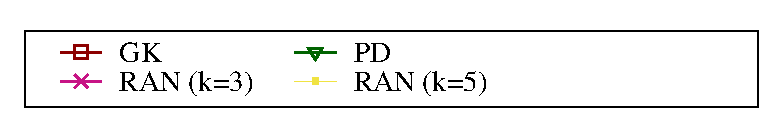
\includegraphics[width=1.0\textwidth]{lambda_legend.eps}
	  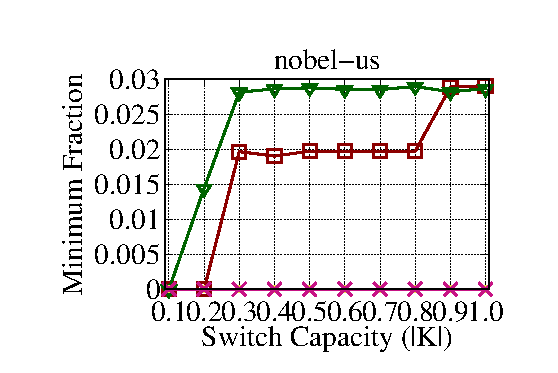
\includegraphics[width=1.0\textwidth]{nobel-us_geni_lambda_e05.eps}
	  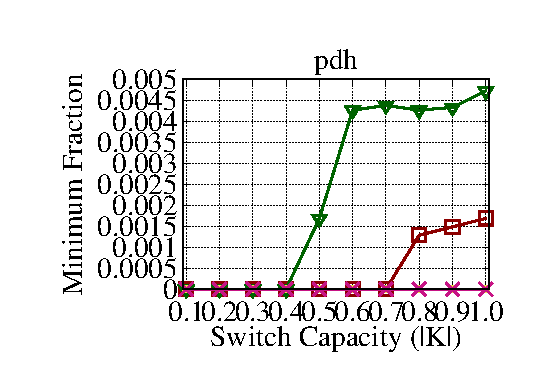
\includegraphics[width=1.0\textwidth]{pdh_geni_lambda_e05.eps}
  \end{figure}
  
  
  
    \begin{figure}[ht]
    \caption{The impact of the switch capacity on the total throughput on GENI.}
	\centering
	  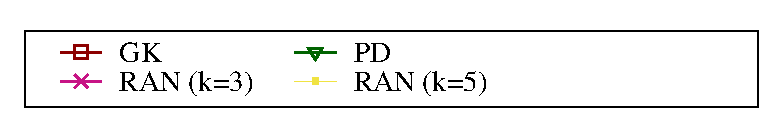
\includegraphics[width=1.0\textwidth]{lambda_legend.eps}
	  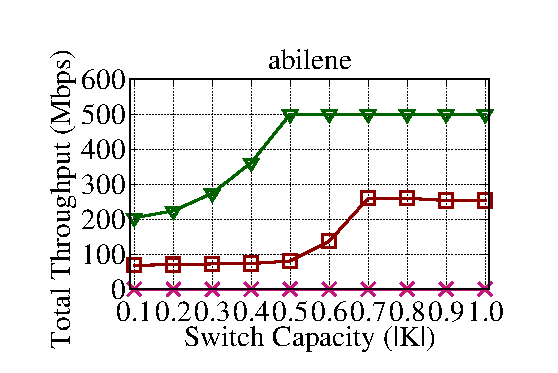
\includegraphics[width=1.0\textwidth]{abilene_geni_throughput_e05.eps}
	  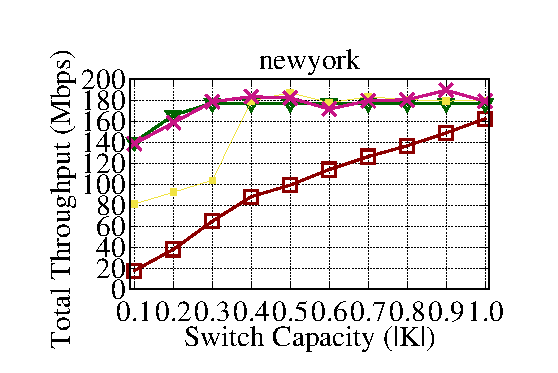
\includegraphics[width=1.0\textwidth]{newyork_geni_throughput_e05.eps}
  \end{figure}
    \begin{figure}[ht]
    \caption{The impact of the switch capacity on the total throughput on GENI.}
	\centering
	  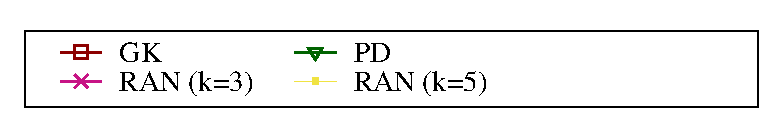
\includegraphics[width=1.0\textwidth]{lambda_legend.eps}
	  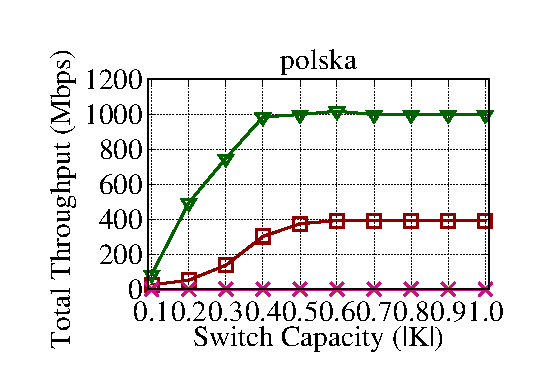
\includegraphics[width=1.0\textwidth]{polska_geni_throughput_e05.eps}
	  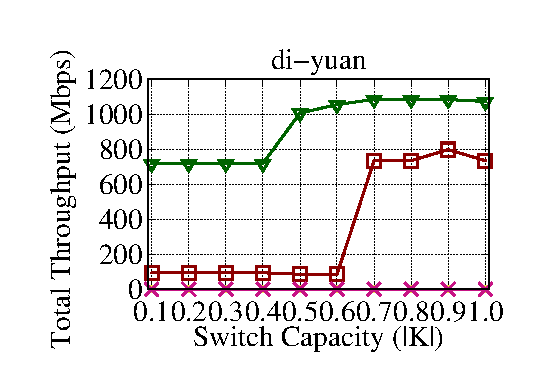
\includegraphics[width=1.0\textwidth]{di-yuan_geni_throughput_e05.eps}
  \end{figure}
  \begin{figure}[ht]
    \caption{The impact of the switch capacity on the total throughput on GENI.}
	\centering
	  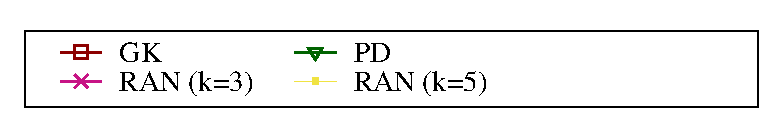
\includegraphics[width=1.0\textwidth]{lambda_legend.eps}
	  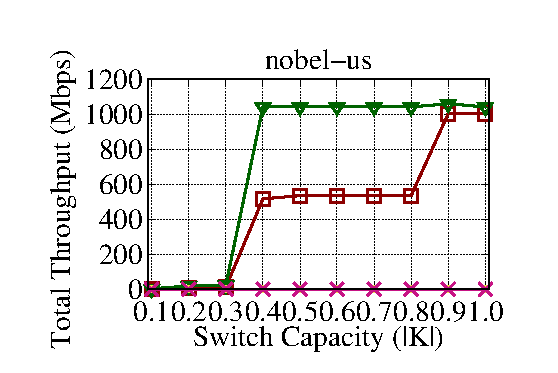
\includegraphics[width=1.0\textwidth]{nobel-us_geni_throughput_e05.eps}
	  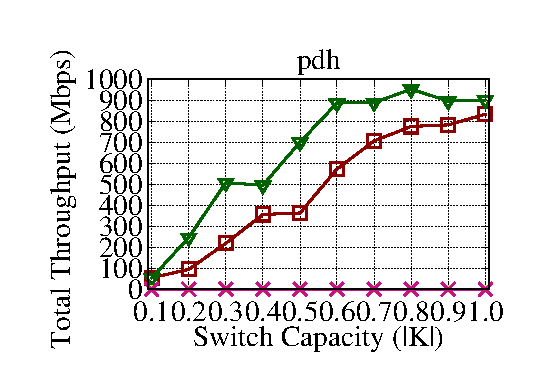
\includegraphics[width=1.0\textwidth]{pdh_geni_throughput_e05.eps}
  \end{figure}
  \chapter{Summary}
    \section{conclusion}
    \qquad For implementing a routing algorithm of SDN, GENI is a persuasive environment for experiment compared to simulator like NS-2, mininet, ... . In this thesis, we divided the algorithms into online algorithm and offline algorithm. For each part, we gave a full description about how to implement it in GENI.  Reader could base on this thesis to get a faster way for building their experiment. 
  \begin{thebibliography}{1}
\bibitem{iperf}
    iPerf, \emph{https://iperf.fr/}.
\bibitem{our}
    Tzu-Wen Chang, Yao-Jen Tang, Ming-Jer Tsai, \emph{Efficient Algorithm for Maximum Concurrent Flow Problem in MPLS-based Software Defined Networks}.
 
\bibitem{grag}
    N. Garg and J. Könemann. \emph{“Faster and simpler algorithms for multicom-modity flow and other fractional packing problems,”} SIAM Journal on
Computing, 2007.
\bibitem{gk}
	A. Gushchin, A. Walid, and A. Tang, “Enabling service function chaining
through routing optimization in software defined networks,” in IEEE
Allerton Conference on Communication, Control, and Computing, 2015.
\bibitem{SNDlib}
	S. Orlowski, R. Wessäly, M. Pióro, and A. Tomaszewski, “Sndlib 1.0-
survivable network design library,” Networks, 2010. [Online]. Available:
http://sndlib.zib.de
\end{thebibliography}
  \end{large}
  \end{document}